%%%%%%%%%%%%%%%%%%%%%%%%%%%%%%%%%%%%%%%%%
% Short Sectioned Assignment LaTeX Template Version 1.0 (5/5/12)
% This template has been downloaded from: http://www.LaTeXTemplates.com
% Original author:  Frits Wenneker (http://www.howtotex.com)
% License: CC BY-NC-SA 3.0 (http://creativecommons.org/licenses/by-nc-sa/3.0/)
%%%%%%%%%%%%%%%%%%%%%%%%%%%%%%%%%%%%%%%%%

%----------------------------------------------------------------------------------------
%	PACKAGES AND OTHER DOCUMENT CONFIGURATIONS
%----------------------------------------------------------------------------------------

\documentclass[paper=a4, fontsize=11pt]{scrartcl} % A4 paper and 11pt font size

% ---- Entrada y salida de texto -----

\usepackage[T1]{fontenc} % Use 8-bit encoding that has 256 glyphs
\usepackage[utf8]{inputenc}
\usepackage{fourier} % Use the Adobe Utopia font for the document - comment this line to return to the LaTeX default

% ---- Idioma --------

\usepackage[spanish, es-tabla]{babel} % Selecciona el español para palabras introducidas automáticamente, p.ej. "septiembre" en la fecha y especifica que se use la palabra Tabla en vez de Cuadro

% ---- Otros paquetes ----
\usepackage{array}
\usepackage{multirow}
\usepackage[dvipsnames]{xcolor}
\usepackage{url} % ,href} %para incluir URLs e hipervínculos dentro del texto (aunque hay que instalar href)
\usepackage{amsmath,amsfonts,amsthm, tikz,dsfont} % Math packages
\usepackage[hidelinks]{hyperref}
%\usepackage{graphics,graphicx, floatrow} %para incluir imágenes y notas en las imágenes
\usepackage{graphics,graphicx, float, listings} %para incluir imágenes y colocarlas

% Para hacer tablas comlejas
%\usepackage{multirow}
%\usepackage{threeparttable}

%\usepackage{sectsty} % Allows customizing section commands
%\allsectionsfont{\centering \normalfont\scshape} % Make all sections centered, the default font and small caps

\usepackage{fancyhdr} % Custom headers and footers
\pagestyle{fancyplain} % Makes all pages in the document conform to the custom headers and footers
\fancyhead{} % No page header - if you want one, create it in the same way as the footers below
\fancyfoot[L]{} % Empty left footer
\fancyfoot[C]{} % Empty center footer
\fancyfoot[R]{\thepage} % Page numbering for right footer
\renewcommand{\headrulewidth}{0pt} % Remove header underlines
\renewcommand{\footrulewidth}{0pt} % Remove footer underlines
\setlength{\headheight}{13.6pt} % Customize the height of the header

\numberwithin{equation}{section} % Number equations within sections (i.e. 1.1, 1.2, 2.1, 2.2 instead of 1, 2, 3, 4)
\numberwithin{figure}{section} % Number figures within sections (i.e. 1.1, 1.2, 2.1, 2.2 instead of 1, 2, 3, 4)
\numberwithin{table}{section} % Number tables within sections (i.e. 1.1, 1.2, 2.1, 2.2 instead of 1, 2, 3, 4)

\setlength\parindent{0pt} % Removes all indentation from paragraphs - comment this line for an assignment with lots of text

\newcommand{\horrule}[1]{\rule{\linewidth}{#1}} % Create horizontal rule command with 1 argument of height


%----------------------------------------------------------------------------------------
%	TÍTULO Y DATOS DEL ALUMNO
%----------------------------------------------------------------------------------------

\title{	
\normalfont \normalsize 
\textsc{\textbf{Modelos de computación (2016-2017)} \\ Grado en Ingeniería Informática \\ Universidad de Granada} \\ [25pt] % Your university, school and/or department name(s)
\horrule{0.5pt} \\[0.4cm] % Thin top horizontal rule
\huge Memoria de practicas \\ % The assignment title
\horrule{2pt} \\[0.5cm] % Thick bottom horizontal rule
\begin{figure}[H] %con el [H] le obligamos a situar aquí la figura
	\centering
	
\includegraphics[scale=0.5]{image/ugr.png}  %el parámetro scale permite agrandar o achicar la imagen. En el nombre de archivo puede especificar directorios
\end{figure}
}

\author{Antonio Rodríguez Alaminos} % Nombre y apellidos

\date{\normalsize\today} % Incluye la fecha actual

%----------------------------------------------------------------------------------------
% DOCUMENTO
%----------------------------------------------------------------------------------------

\begin{document}

%----------------------------------------------------------------------------------------
% PORTADA
%----------------------------------------------------------------------------------------

\maketitle % Muestra el Título

\newpage %inserta un salto de página

\tableofcontents % para generar el índice de contenidos

%----------------------------------------------------------------------------------------
% INDICE
%----------------------------------------------------------------------------------------

\listoffigures

\listoftables

\newpage

%----------------------------------------------------------------------------------------
% CUESTION 1
%----------------------------------------------------------------------------------------
\section{Práctica 1}

\subsection{Ejercicio 1} 

\textit{Describir el lenguaje generado por las siguientes gramáticas en \{0, 1\}*.}

\subsubsection{Apartado A} 

\textit{$ S \rightarrow 0 S_{1} 1 \hspace{3cm} S_{1} \rightarrow 0S_{1} | 1S_{1} | \epsilon\ $} \newline

Cuando tenemos que $ S_{1} \rightarrow \epsilon $ : \newline
$ S \rightarrow 0 S_{1} 1 \Rightarrow 0 \epsilon 1 \Rightarrow \textbf{01} $ \newline

Ahora comprobamos cuando $ S_{1} \rightarrow 0S_{1} $ : \newline
$ S \rightarrow 0 S_{1} 1 \rightarrow 0 0 S_{1} 1 \rightarrow 0 0 0 S_{1} 1 \rightarrow \textbf{00000...1} $ \newline

Continuamos cuando $ S_{1} \rightarrow 1S_{1} $ : \newline
$ S \rightarrow 0 S_{1} 1 \Rightarrow 0 1S_{1}  1 \Rightarrow 0 1S_{1}  1 1 \Rightarrow \textbf{0...11111} $ \newline

Y por ultimo cuando tenemos que $ S_{1} \rightarrow 1S_{1} $ o $ S_{1} \rightarrow 0S_{1} $: \newline
$ S \rightarrow 0 S_{1} 1 \Rightarrow 0 1S_{1}  1 \Rightarrow 0 1S_{1}  1 1  \Rightarrow 0 S_{1} 1 1 1 \Rightarrow 0 0 0 S_{1} 1 1 1 \Rightarrow \textbf{0...0101...1010...1} $ \newline

Por lo tanto tenemos que $ L_{n}=\{0u1 \; tq \; u \in \{0.1\}^{*} \} $

\subsubsection{Apartado B} 

\textit{$ S \rightarrow S_{1} 101 S_{1} \hspace{3cm} S_{1} \rightarrow 0S_{1} | 1S_{1} | \epsilon $ }\newline

Aplicamos los mismos pasos del ejercicio anterior, empezamos con $ S_{1} \rightarrow \epsilon $ : \newline
$ S \rightarrow S_{1} 1 0 1 S_{1} \Rightarrow \epsilon 1 0 1 \epsilon \Rightarrow \textbf{101} $ \newline

Ahora comprobamos cuando $ S_{1} \rightarrow 0S_{1} $ : \newline
$ S \rightarrow S_{1} 1 0 1 S_{1} \Rightarrow 0S_{1} 1 0 1 0S_{1} \Rightarrow 0S_{1} 0 1 0 1 0 0S_{1} \Rightarrow \textbf{00000...101...00000} $ \newline

Continuamos cuando $ S_{1} \rightarrow 1S_{1} $ : \newline
$ S \rightarrow S_{1} 1 0 1 S_{1} \Rightarrow 1S_{1} 1 0 1 1S_{1} \Rightarrow 1S_{1} 1 1 0 1 1 1S_{1} \Rightarrow \textbf{11111...101...11111} $ \newline

Y por ultimo cuando tenemos que $ S_{1} \rightarrow 1S_{1} $ o $ S_{1} \rightarrow 0S_{1} $: \newline
$ S \rightarrow S_{1} 1 0 1 S_{1} \Rightarrow 1S_{1} 1 0 1 1S_{1} \Rightarrow 1S_{1} 1 1 0 1 1 1S_{1} \Rightarrow 0S_{1}11 1 0 111 0S_{1} \Rightarrow 0S_{1} 0 111 0 111 0 0S_{1} \Rightarrow \textbf{0101....101...1010} $ \newline

Por lo tanto tenemos que $ L_{n}=\{ u 101 v \; tq \; u,v \in \{0.1\}^{*} \} $

\newpage

\subsubsection{Apartado C} 

$ S \rightarrow 0S_{1} | S_{1} \hspace{1.5cm} || \hspace{1.5cm} S_{1} \rightarrow 1S_{1}0 | 1S_{2}0 \hspace{1.5cm} || \hspace{1.5cm} S_{2} \rightarrow 0S_{2}1 | \epsilon  $ \newline

Por lo tanto tenemos que $ L_{n}=\{ 0^{i} \; 1^{j} \; 0^{k} \; 1^{k} \; 0^{j}  \; tq \; i \in [0,1], \; j \ge 1, \; k \ge 0 \} $

\subsection{Ejercicio 2}

\textit{Encontrar gramáticas de tipo 2 para los siguientes lenguajes sobre el alfabeto \{0,1\}. En cada caso determinar si los lenguajes generados son de tipo 3, estudiando si existe una gramática de tipo 3 que los genera.}

\subsubsection{Apartado A} 

\textit{Palabras que comienzan con la subcadena “10” y acaban en “001”.}

\begin{itemize}
	\item \textbf{Tipo 2} \newline
	$ G = \{ S, \{ A \} , \{ 01 \}  ,P,S\} $ \newline
	$ P = \{ S \rightarrow 10A001 \hspace{1cm} A \rightarrow 1A \hspace{1cm} A \rightarrow 0A \hspace{1cm} A \rightarrow \epsilon \} $
	\item \textbf{Tipo 3} \newline
	$ G = \{ S, \{ S_{1},S_{2} \} , \{ 01 \}  ,P,S\} $ \newline
	$ P = \{ S \rightarrow 10S_{1} | S_{2} \hspace{1cm} S_{1} \rightarrow 1S_{1}|0S_{1}|S_{2} \hspace{1cm} S_{2} \rightarrow 001 \} $
\end{itemize}

\subsubsection{Apartado B} 

\textit{Palabras que tienen 2 o 3 “0”.}

\begin{itemize}
	\item \textbf{Tipo 2} \newline
	$ G = \{ S, \{ A,B,C \} , \{ 01 \}  ,P,S\} $ \newline
	$ P = \{ S \rightarrow 1S|0S_{1}|0S_{3}0 \hspace{1cm} S_{1} \rightarrow 1S_{1}|0S_{2}|0S_{3} \hspace{1cm} S_{2} \rightarrow 1S_{2}|0S_{3} \hspace{1cm} S_{3} \rightarrow \epsilon \} $
	\item \textbf{Tipo 3} \newline
	$ G = \{ S, \{ A,B,C \} , \{ 01 \}  ,P,S\} $ \newline
	$ P = \{ S \rightarrow 1A \hspace{1cm} S \rightarrow 0B \hspace{1cm} A \rightarrow 1A \hspace{1cm} A \rightarrow 0B \hspace{1cm} B \rightarrow 1B \newline  B \rightarrow 0C \hspace{1cm} C \rightarrow 1C \hspace{1cm} C \rightarrow 0D \hspace{1cm} C \rightarrow \epsilon \hspace{1cm} D \rightarrow 1D \hspace{1cm} D \rightarrow \epsilon\} $
\end{itemize}

\subsubsection{Apartado C} 

\textit{Palabras que no contienen la subcadena “011”.}

\begin{itemize}
	\item \textbf{Tipo 3} \newline
	$ G = \{ S, \{ A,B \} , \{ 01 \}  ,P,S\} $ \newline
	$ P = \{ S \rightarrow 1S \hspace{1cm} S \rightarrow 0A \hspace{1cm} S \rightarrow \epsilon \hspace{1cm} A \rightarrow 0A \hspace{1cm} A \rightarrow 1B \newline  A \rightarrow \epsilon \hspace{1cm} B \rightarrow 0S \hspace{1cm} B \rightarrow \epsilon \} $
\end{itemize}

\newpage

\subsection{Ejercicio 3}

\textit{Como empleado de la empresa de desarrollo de videojuegos “MoreThanDungeons”, se le ha pedido diseñar una gramática que represente los niveles de un juego de exploración de mazmorras y las salas de estas, con una serie de restricciones.} \newline

\textit{En cada nivel:} 

\begin{itemize}

	\item \textit{Existen salas grandes (g) y pequeñas (p) que deberán ser limpiadas de monstruos para avanzar. (Los niveles más sencillos tienen al menos una sala grande)}
	\item \textit{Hay al menos una sala de tendero (t), donde recuperar fuerzas y comprar objetos.}
	\item \textit{Habrá una sola sala secreta (x), siempre le precede una sala grande. Es decir, siempre habrá una “g” delante de “x”.}
	\item \textit{Cada nivel de la mazmorra debe acabar con una sala final de jefe (j).}
\end{itemize}

\textit{Por ejemplo, la cadena terminal “ppgxtj” representa el nivel en el que el jugador debe de pasar por dos habitaciones pequeñas “pp”, seguidas de una grande “g”. En esta, podrá encontrar la sala secreta “x”. A continuación, podrá recuperar fuerzas en la tienda “t”. Para finalmente, enfrentarse al jefe final “j” del nivel.} \newline

\textit{Elabore una gramática que genere estos niveles con sus restricciones. Cada palabra del lenguaje es UN SOLO NIVEL. ¿A qué tipo de la jerarquía de Chomsky pertenece la gramática que ha diseñado?} \newline

$ G = \{S,  A, \{ g,x,t,p \} ,P,S\} $ \newline
$ P = \{ S \rightarrow AtAgxAj \hspace{1cm} A \rightarrow gA \hspace{1cm} A \rightarrow pA \hspace{1cm} A \rightarrow tA \hspace{1cm} A \rightarrow \epsilon \} $ \newline

\textit{¿Podría diseñar una gramática de tipo 3 para dicho problema?} \newline

$ G = \{S,  A, \{ g,x,t,p \} ,P,S\} $ \newline
$ P = \{ S \rightarrow gS|pS|tS_{1}|gxS_{2} \hspace{1cm} S_{1} \rightarrow gS_{1}|pS_{1}|tS_{1}|gxS_{3} \hspace{1cm} S_{2} \rightarrow gS_{2}|pS_{2}|tS_{3} \newline S_{3} \rightarrow gS_{3}|pS_{3}|tS_{3}|j \} $ \newline

\newpage

\section{Practica 2}

\subsection{Ejercicio 1}

\textit{Construir un AFD que acepte cada uno de los siguientes lenguajes con alfabeto \{a,b\}:}

\subsubsection{Apartado A}

\textit{El lenguaje de las palabras que contienen la subcadena aaa.}

\begin{figure}[h]
\centering
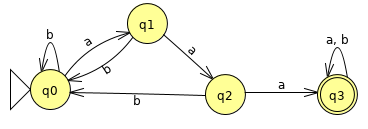
\includegraphics[width=0.7\linewidth]{image/ejercicio1}
\caption[prac 2 - ejer 1A]{Grafo del ejercicio 1A}
\label{fig:ejercicio1A}
\end{figure}

\subsubsection{Apartado B}

\textit{El lenguaje de las palabras que empiezan o terminan (o ambas cosas) en aaa.}

\begin{figure}[h]
	\centering
	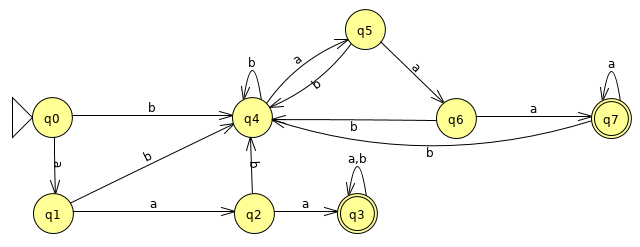
\includegraphics[width=1\linewidth]{image/ejercicio2}
	\caption[prac 2 - ejer 1B]{Grafo del ejercicio 1B}
	\label{fig:ejercicio1B}
\end{figure}

\newpage

\subsubsection{Apartado C}

\textit{El lenguaje formado por las cadenas donde el número de a’s es divisible por 3.}

\begin{figure}[h]
	\centering
	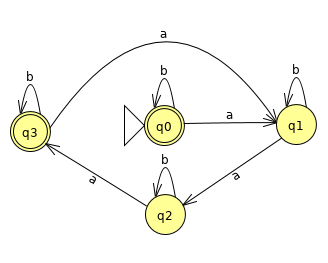
\includegraphics[width=0.6\linewidth]{image/ejercicio3}
	\caption[prac 2 - ejer 1C]{Grafo del ejercicio 1C}
	\label{fig:ejercicio1C}
\end{figure}

\subsection{Ejercicio 2}

\textit{Construir un AFND que acepte cada uno de los siguientes lenguajes con alfabeto \{a,b\}:}

\subsubsection{Apartado A}

\textit{El lenguaje de las palabras que terminan en aaa.}

\begin{figure}[h]
	\centering
	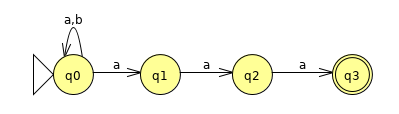
\includegraphics[width=0.6\linewidth]{image/ejercicio4}
	\caption[prac 2 - ejer 2A]{Grafo del ejercicio 2A}
	\label{fig:ejercicio2A}
\end{figure}

\newpage

\subsubsection{Apartado B}

\textit{El lenguaje de las palabras que empiezan o terminan (o ambas cosas) en aaa.}

\begin{figure}[h]
	\centering
	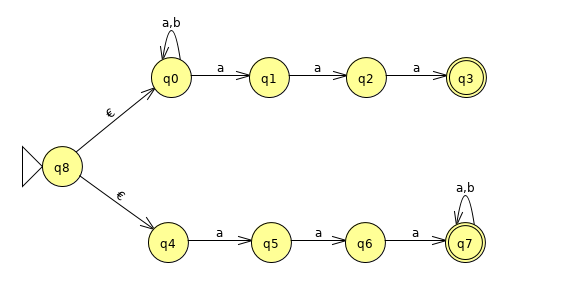
\includegraphics[width=0.8\linewidth]{image/ejercicio5}
	\caption[prac 2 - ejer 2B]{Grafo del ejercicio 2B}
	\label{fig:ejercicio2B}
\end{figure}

\subsubsection{Apartado C}

\textit{El lenguaje de las palabras que contengan, simultáneamente, las subcadenas aba y abb. \newline
Este AFND también acepta cadenas en la que estas subcadenas están solapadas (por ejemplo, las palabras “ababb” y “aaabbbaba” serían aceptadas).}

\begin{figure}[H]
	\centering
	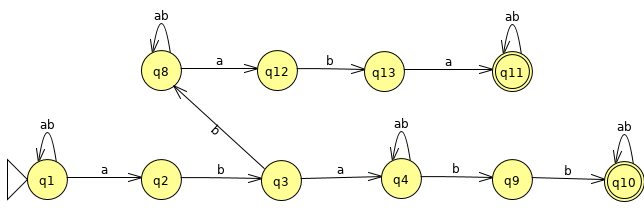
\includegraphics[width=1\linewidth]{image/ejercicio6}
	\caption[prac 2 - ejer 2C]{Grafo del ejercicio 2C}
	\label{fig:ejercicio2C}
\end{figure}

\newpage

\subsection{Ejercicio 3}

\textit{Diseñar una Máquina de Mealy o de Moore que, dada una cadena usando el alfabeto A={‘a’, ‘w’, ‘o’}, encienda un led verde (salida ‘V’) cada vez que se detecte la cadena “woow” en la entrada, apagándolo cuando lea cualquier otro símbolo después de esta cadena (representamos el led apagado con la salida“X“). El autómata tiene que encender el led verde (salida ‘V’) , tantas
veces como aparezca en la secuencia “woow” en la entrada, y esta secuencia puede estar solapada. Por ejemplo, ante la siguiente entrada, la Máquina de Mealy/Moore emitirá la salida:}

\begin{table}[H]
	\centering
	\begin{tabular}[scale 0.3]{|c|c|}
		\hline
		\textbf{Entrada} & aaawoawoowoowwoowa \\
		\hline
		\textbf{Salida} & XXXXXXXXXVXXVXXXVX \\
		\hline
	\end{tabular}  
\end{table}

\begin{figure}[H]
	\centering
	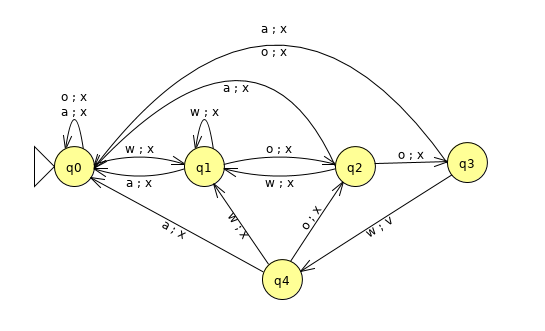
\includegraphics[width=1\linewidth]{image/ejercicio7}
	\caption[prac 2 - ejer 2C]{Grafo del ejercicio 3}
	\label{fig:ejercicio3}
\end{figure}

\newpage

\subsection{Ejercicio 4}

\textit{Obtener un AFD equivalente al AFND siguiente:}

\begin{figure}[H]
\centering
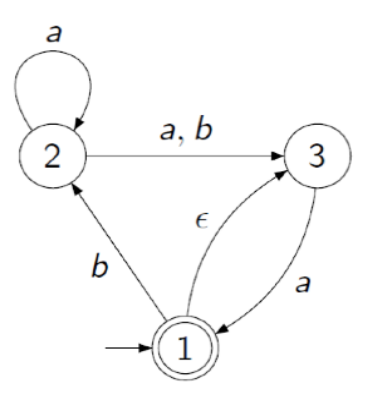
\includegraphics[width=0.3\linewidth]{image/ejercicio04}
\end{figure}

\begin{table}[H]
	\centering
	\begin{tabular}[scale 0.3]{|c|c|c|}
		\hline
		\textbf{Estado/Atributo} & a & b \\
		\hline \hline
		$ q_{1} q_{3} $ & $ q_{1} q_{3} $ & $ q_{2} $ \\
		\hline
		$ q_{2} $ & $ q_{2} q_{3} $ & $ q_{3} $ \\
		\hline
		$ q_{2} q_{3} $ & $ q_{2} q_{3} q_{1} $ & $ q_{3} $ \\
		\hline
		$  q_{2} q_{3} q_{1} $ & $  q_{2} q_{3} q_{1} $ & $ q_{3} q_{2} $ \\
		\hline
		$ q_{3} $ & $ q_{1} q_{3} $ & $ \emptyset $ \\
		\hline		
	\end{tabular} 
	 \caption[prac 2 - ejer 2C]{Caminos, ejercicio 4}
\end{table}

\begin{figure}[H]
	\centering
	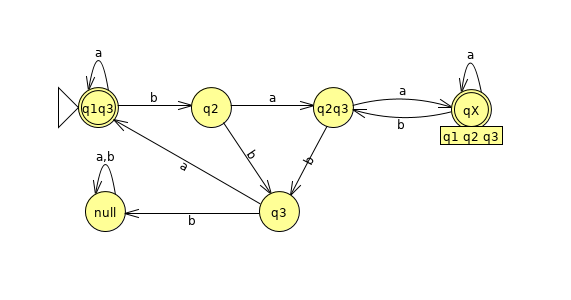
\includegraphics[width=1\linewidth]{image/ejercicio8}
	\caption[prac 2 - ejer 2C]{Grafo del ejercicio 4}
	\label{fig:ejercicio45}
\end{figure}

\newpage

\section{Practica 3}

\subsection{Ejercicio 1}

\textit{Pensar un problema original de procesamiento de textos. Para la resolución de este problema debe ser apropiado el uso de Lex, o sea, se debe resolver mediante el emparejamiento de cadenas con expresiones regulares y la asociación de acciones a cada emparejamiento. Se presentará una descripción por escrito del problema. Consultar al profesor de prácticas acerca de la complejidad del problema propuesto.} \newline

El problema real que voy a resolver, trata en obtener: las cadenas que tienen la información relevante sobre los log obtenidos tras una investigación de clasificación sobre datos no balanceados.

\subsection{Ejercicio 2}

\textit{Resolver el problema propuesto usando Lex.} \newline

Código del autómata en lex. \newline

 \lstset{language=C, breaklines=true, basicstyle=\footnotesize}
	 \begin{lstlisting}[frame=single]
	 
	     /*----- Seccion de Declaraciones -----*/
     
     %{
     
	     #include <stdio.h>
	     #include <string.h>
	     #include <stdbool.h>
	     
	     int tiempoIntervalo = 0;
	     int tiempo = 0;
	     int contador = 1;
	     char charTimeInit[11];
	     char charTimeEnd[11];
	     void escribirNombre(char* dato1, int tam);
	     void escribirInicio(char* dato1, int tam);
	     void escribirFin(char* dato1, int tam);
     
     %}
     
     initTime            ("*** BEGIN OF EXPERIMENT ")
     fechaDia            {initTime}([a-zA-Z]{3})
     fechaMes            {fechaDia}.([a-zA-Z]{3})
     fechaDiaNum         {fechaMes}.([0-9]{2})
     hora                {fechaDiaNum}.([0-9]{2}\:[0-9]{2}\:[0-9]{2})
     cet                 {hora}.([a-zA-Z]{3})
     initProceso         {cet}.([0-9]{4})
     
     initNombre           ("The name is: ")
     nombreProceso       {initNombre}([a-zA-Z]+).([a-zA-Z]+)* 
     
     endTime             ("*** END OF EXPERIMENT ")
     endfechaDia         {endTime}([a-zA-Z]{3})
     endfechaMes         {endfechaDia}.([a-zA-Z]{3})
     endfechaDiaNum      {endfechaMes}.([0-9]{2})
     endhora             {endfechaDiaNum}.([0-9]{2}\:[0-9]{2}\:[0-9]{2})
     endcet              {endhora}.([a-zA-Z]{3})
     endProceso          {endcet}.([0-9]{4})
     
     %%
     
	     /*----- Seccion de Reglas -----*/
     
     {initProceso}               { escribirInicio(yytext, yyleng); } 
     {nombreProceso}             { escribirNombre(yytext, yyleng); } 
     {endProceso}                { escribirFin(yytext, yyleng); } 
     .                           {}
     \n                          {}
     
     %%
     
	     /*----- Seccion de Procedimientos -----*/
     
     int main (int argc, char *argv[]){
	     if (argc == 2)  {
		     yyin = fopen (argv[1], "rt");
		     
		     if (yyin == NULL)    {
			     printf ("El fichero %s no se puede abrir\n", argv[1]);
			     exit (-1);
		     }
	     }
	     else yyin = stdin;
	     
	     yylex ();
	     printf ("\n");
	     printf ("\n --> Tiempo Final: %is", tiempo);
	     printf ("\n");
	     
	     return 0;
     }
     
     void escribirInicio(char* dato1, int tam){
	     char* tipo = "Inicio: ";
	     char* aux;
	     char letra;
	     int tamanio = 32;
	     
	     printf ("\n## Inicio Proceso: %i ## \n", contador);
	     printf ("\n%s",tipo);
	     
	     aux = dato1;
	     
	     for(int i=24; i < strlen(dato1); i++){
		     letra = dato1[i];
		     printf ("%c",letra);
	     }
	     
	     for(int i=0; i < 11; i++){
		     letra = aux[tamanio];
		     charTimeInit[i] = letra;
		     tamanio++;
	     }
     }
     
     void escribirFin(char* dato1, int tam){
	     char* tipo = "Fin: ";
	     char letra;
	     char* aux;
	     int tamanio = 30;
	     
	     if (tieneNombre != true){
		     printf ("\nNombre: No tiene nombre. ");
	     }
	    
	     printf ("\n%s",tipo);
	     
	     aux = dato1;
	     
	     for(int i=22; i < strlen(dato1); i++){
		     letra = dato1[i];
		     printf ("%c",letra);
	     }
	     
	     for(int i=0; i < 11; i++){
		     letra = aux[tamanio];
		     charTimeEnd[i] = letra;
		     tamanio++;
	     }
	     
	     tiempoTotal();
	     
	     printf ("\n \n## Fin Proceso: %i ## \n \n################################# \n", contador);
	     \\
	     
	     tieneNombre = false;
	       
	     contador++;
     }
     
     void escribirNombre(char* dato1, int tam){
	     char* tipo = "Nombre: ";
	     char letra;
	     
	     printf ("\n%s",tipo);
	     
	     for(int i=13; i < strlen(dato1); i++){
		     letra = dato1[i];
		     printf ("%c",letra);
	     }
	     
	     tieneNombre = true;
     }
     
     void tiempoTotal(){
	     int tamanio = 0, tiempoTotalInit = 0, tiempoTotalEnd = 0;
	     char CdiaInit[2], CdiaEnd[2], ChoraInit[2], ChoraEnd[2], CminInit[2], CminEnd[2], CsegInit[2], CsegEnd[2];
	     
	     for(int i = 0; i < 2; i++){
		     CdiaInit[i] = charTimeInit[tamanio];
		     CdiaEnd[i] = charTimeEnd[tamanio];
		     tamanio++;
	     }
	     
	     tamanio++;
	     
	     for(int i = 0; i < 2; i++){
		     ChoraInit[i] = charTimeInit[tamanio];
		     ChoraEnd[i] = charTimeEnd[tamanio];
		     tamanio++;
	     }
	     
	     tamanio++;
	     
	     for(int i = 0; i < 2; i++){
		     CminInit[i] = charTimeInit[tamanio];
		     CminEnd[i] = charTimeEnd[tamanio];
		     tamanio++;
	     }
	     
	     tamanio++;
	     
	     for(int i = 0; i < 2; i++){
		     CsegInit[i] = charTimeInit[tamanio];
		     CsegEnd[i] = charTimeEnd[tamanio];
		     tamanio++;
	     }
	     
	     tiempoTotalInit = atoi(CdiaInit)*24*60*60;
	     tiempoTotalInit += atoi(ChoraInit)*60*60;
	     tiempoTotalInit += atoi(CminInit)*60;
	     tiempoTotalInit += atoi(CsegInit);
	     
	     tiempoTotalEnd = atoi(CdiaEnd)*24*60*60;
	     tiempoTotalEnd += atoi(ChoraEnd)*60*60;
	     tiempoTotalEnd += atoi(CminEnd)*60;
	     tiempoTotalEnd += atoi(CsegEnd);
	     
	     tiempoIntervalo = tiempoTotalEnd - tiempoTotalInit;
	     
	     tiempo += tiempoIntervalo;
	     
	     printf ("\n   --> Tiempo Proceso: %is", tiempoIntervalo);
     }
    
	 \end{lstlisting}
	 
	 Enlaces de descarga:
	 \begin{itemize}
	 	\item  \href{https://www.dropbox.com/s/hopkh3n6ucnwzmk/automataIN.l?dl=0}{ \textcolor{blue}{Automata lex.}}
	 	\item  \href{https://www.dropbox.com/s/jybcbsmnqem10nn/log-prueba20?dl=0}{ \textcolor{blue}{Prueba 1}}
	 	\item  \href{https://www.dropbox.com/s/1035oj3gs0gvl8d/log-prueba14?dl=0}{ \textcolor{blue} {Prueba 2} }
	 	\item  \href{https://www.dropbox.com/s/cl5v90zl3yn1u9i/p?dl=0}{ \textcolor{blue} {Resultado} }
	 \end{itemize}
	 
\subsection{Ejercicio 3}

\textit{Realizar un documento presentando el problema y la solución con Lex.} \newline

El principal problema que tiene el extraer esta información sin ayuda de los autómatas es la cantidad de tiempo y lo compleja que encontrarla entre mas de 45000 de líneas de código. \newline

Solución obtenida con el autómatas en diversos casos:

\begin{itemize}
	\item \textbf{Prueba 20} \newline
	
	\#\# Inicio Proceso: 1 \#\# \newline \newline
	
	Inicio: Fri Jan 06 00:51:34 CET 2017\newline
	Nombre: IterativePartitioningFilter\newline
	Fin: Fri Jan 06 01:14:07 CET 2017\newline
	--> Tiempo Proceso: 1353s\newline \newline
	
	\#\# Fin Proceso: 1 \#\# \newline \newline
	
	\#\#\#\#\#\#\#\#\#\#\#\#\#\#\#\#\#\#\#\#\#\#\#\#\#\#\#\#\#\#\#\#\# \newline \newline
	
	\#\# Inicio Proceso: 2 \#\# \newline
	
	Inicio: Fri Jan 06 01:14:07 CET 2017\newline
	Nombre: IterativePartitioningFilter\newline
	Fin: Fri Jan 06 01:36:40 CET 2017\newline
	--> Tiempo Proceso: 1353s\newline \newline
	
	\#\# Fin Proceso: 2 \#\# \newline
	
	\#\#\#\#\#\#\#\#\#\#\#\#\#\#\#\#\#\#\#\#\#\#\#\#\#\#\#\#\#\#\#\#\# \newline
	
	............\newline
	
	\#\#\#\#\#\#\#\#\#\#\#\#\#\#\#\#\#\#\#\#\#\#\#\#\#\#\#\#\#\#\#\#\# \newline \newline
	
	\#\# Inicio Proceso: 31 \#\# \newline \newline
	
	Inicio: Fri Jan 06 03:29:08 CET 2017 \newline
	Nombre: No tiene nombre. \newline
	Fin: Fri Jan 06 03:29:08 CET 2017\newline
	--> Tiempo Proceso: 0s\newline \newline
	
	\#\# Fin Proceso: 31 \#\# \newline \newline
	
	\#\#\#\#\#\#\#\#\#\#\#\#\#\#\#\#\#\#\#\#\#\#\#\#\#\#\#\#\#\#\#\#\# \newline \newline \newline
	
	
	--> Tiempo Final: 9454s \newline
	
\end{itemize}

\newpage

\section{Practica 4}

\subsection{Ejercicio 1}

\textit{Determinar cuáles de las siguientes gramáticas son ambiguas y, en su caso, comprobar si los lenguajes generados son inherentemente ambiguos, Justificar la respuesta.}

\subsubsection{Apartado A}

$ S \rightarrow 01S \; | \; 010S \; | \; 101S \; | \; \epsilon $ \newline

Como por norma las gramáticas de tipo 3 no son ambiguas podemos decir que esta al serlo no puede ser ambigua. \newline

\subsubsection{Apartado B}
	
$ S \rightarrow 0S1 \; | \; S1 \; | \; 0S \; | \; 0 $ 	\newline

\begin{center}
	Palabra 0011 \hspace{2.5cm} Palabra 0011
\end{center}
\begin{center}	
	\begin{tikzpicture}{r}[h]
	\node {$S$} 
	child {node {$0$}}
	child {node {$S$}
		child {node {$S$}
			child {node {$0$}}
			}
		child {node {$1$}}
		}
	child {node {$1$}}
	;
	\end{tikzpicture}
	\hspace{2cm}
	\begin{tikzpicture}{r}[h]
	\node {$S$} 
	child {node {$0$}}
	child {node {$S$}
		child {node {$S$}
			child {node {$S$}
				child {node {$0$}}}
			child {node {$1$}}
		}
		child {node {$1$}}
	}
	;
	\end{tikzpicture}
\end{center}		

Como tenemos dos grafos que dan la misma palabra podemos decir que la gramática es ambigua. Y como podemos encontrar la gramática $ S \rightarrow S1|S0|0 $ , diremos también que es inherentemente ambigua.

\newpage

\subsubsection{Apartado C}
	
$ S \rightarrow A1B \hspace{2.5cm} A \rightarrow 0A \; | \; \epsilon \hspace{2.5cm} B \rightarrow  0B \; | \; 1B \; | \; \epsilon $ \newline

Como podemos ver a simple vista, las S generan A por la izquierda y B por la derecha por lo que nunca podremos encontrar dos arboles iguales. Esto nos dice que la gramática no es ambigua y por lo tanto el lenguaje no puede ser inherentemente ambiguo.
\subsection{Ejercicio 2}

\textit{Eliminar símbolos y producciones inútiles. Realizar el procedimiento paso por paso, indicando las variables descartadas y el motivo.} \newline

$ S \rightarrow moA \hspace{2.5cm} S \rightarrow cI \hspace{2.5cm} A \rightarrow  dEs \hspace{2.5cm} A \rightarrow  jBI $ \newline

$ B \rightarrow bb\hspace{2.5cm} B \rightarrow D\hspace{2.5cm} E \rightarrow  elO\hspace{2.5cm} E \rightarrow  Perl$ \newline

$ D \rightarrow de\hspace{2.5cm} C \rightarrow c\hspace{2.5cm} J \rightarrow  kC\hspace{2.5cm} I \rightarrow  fl$ \newline

$ O \rightarrow o\hspace{2.5cm} P \rightarrow ola$ \newline

En primer lugar, eliminaremos las variables que no llegan a las palabras $ T^{*} $ y las producciones donde estas estén: \newline

$ V_{t} = \{ C \} $ \newline

$ S \rightarrow moA \hspace{2.5cm} S \rightarrow cI \hspace{2.5cm} A \rightarrow  dEs \hspace{2.5cm} A \rightarrow  jBI $ \newline

$ B \rightarrow bb\hspace{2.5cm} B \rightarrow D\hspace{2.5cm} E \rightarrow  elO\hspace{2.5cm} E \rightarrow  Perl$ \newline

$ D \rightarrow de\hspace{2.5cm} \textcolor{blue}{ C \rightarrow c} \hspace{2.5cm} J \rightarrow  kC\hspace{2.5cm} I \rightarrow  fl$ \newline

$ O \rightarrow o\hspace{2.5cm} P \rightarrow ola$ \newline \newline

\newpage

$ V_{t} = \{ C,O \} $ \newline

$ S \rightarrow moA \hspace{2.5cm} S \rightarrow cI \hspace{2.5cm} A \rightarrow  dEs \hspace{2.5cm} A \rightarrow  jBI $ \newline

$ B \rightarrow bb\hspace{2.5cm} B \rightarrow D\hspace{2.5cm} E \rightarrow  elO\hspace{2.5cm} E \rightarrow  Perl$ \newline

$ D \rightarrow de\hspace{2.5cm} \textcolor{blue}{ C \rightarrow c} \hspace{2.5cm} J \rightarrow  kC\hspace{2.5cm} I \rightarrow  fl$ \newline

$ \textcolor{blue}{ O \rightarrow o } \hspace{2.5cm} P \rightarrow ola$ \newline \newline

$ V_{t} = \{ C,O,B \} $ \newline

$ S \rightarrow moA \hspace{2.5cm} S \rightarrow cI \hspace{2.5cm} A \rightarrow  dEs \hspace{2.5cm} A \rightarrow  jBI $ \newline

$ \textcolor{blue}{ B \rightarrow bb } \hspace{2.5cm} \textcolor{blue}{ B \rightarrow D } \hspace{2.5cm} E \rightarrow  elO\hspace{2.5cm} E \rightarrow  Perl$ \newline

$ D \rightarrow de\hspace{2.5cm} \textcolor{blue}{ C \rightarrow c} \hspace{2.5cm} J \rightarrow  kC\hspace{2.5cm} I \rightarrow  fl$ \newline

$ \textcolor{blue}{ O \rightarrow o } \hspace{2.5cm} P \rightarrow ola$ \newline \newline

$ V_{t} = \{ C,O,B,D \} $ \newline

$ S \rightarrow moA \hspace{2.5cm} S \rightarrow cI \hspace{2.5cm} A \rightarrow  dEs \hspace{2.5cm} A \rightarrow  jBI $ \newline

$ \textcolor{blue}{ B \rightarrow bb } \hspace{2.5cm} \textcolor{blue}{ B \rightarrow D } \hspace{2.5cm} E \rightarrow  elO\hspace{2.5cm} E \rightarrow  Perl$ \newline

$ \textcolor{blue}{ D \rightarrow de } \hspace{2.5cm} \textcolor{blue}{ C \rightarrow c} \hspace{2.5cm} J \rightarrow  kC\hspace{2.5cm} I \rightarrow  fl$ \newline

$ \textcolor{blue}{ O \rightarrow o } \hspace{2.5cm} P \rightarrow ola$ \newline \newline

$ V_{t} = \{ C,O,B,D,J \} $ \newline

$ S \rightarrow moA \hspace{2.5cm} S \rightarrow cI \hspace{2.5cm} A \rightarrow  dEs \hspace{2.5cm} A \rightarrow  jBI $ \newline

$ \textcolor{blue}{ B \rightarrow bb } \hspace{2.5cm} \textcolor{blue}{ B \rightarrow D } \hspace{2.5cm} E \rightarrow  elO\hspace{2.5cm} E \rightarrow  Perl$ \newline

$ \textcolor{blue}{ D \rightarrow de } \hspace{2.5cm} \textcolor{blue}{ C \rightarrow c} \hspace{2.5cm} \textcolor{blue}{ J \rightarrow  kC } \hspace{2.5cm} I \rightarrow  fl$ \newline

$ \textcolor{blue}{ O \rightarrow o } \hspace{2.5cm} P \rightarrow ola$ \newline \newline

$ V_{t} = \{ C,O,B,D,J,E \} $ \newline

$ S \rightarrow moA \hspace{2.5cm} S \rightarrow cI \hspace{2.5cm} A \rightarrow  dEs \hspace{2.5cm} A \rightarrow  jBI $ \newline

$ \textcolor{blue}{ B \rightarrow bb } \hspace{2.5cm} \textcolor{blue}{ B \rightarrow D } \hspace{2.5cm} \textcolor{blue}{ E \rightarrow  elO } \hspace{2.5cm} \textcolor{blue}{ E \rightarrow  Perl} $ \newline

$ \textcolor{blue}{ D \rightarrow de } \hspace{2.5cm} \textcolor{blue}{ C \rightarrow c} \hspace{2.5cm} \textcolor{blue}{ J \rightarrow  kC } \hspace{2.5cm} I \rightarrow  fl$ \newline

$ \textcolor{blue}{ O \rightarrow o } \hspace{2.5cm} P \rightarrow ola$ \newline \newline

$ V_{t} = \{ C,O,B,D,J,E,A \} $ \newline

$ S \rightarrow moA \hspace{2.5cm} S \rightarrow cI \hspace{2.5cm} \textcolor{blue}{ A \rightarrow  dEs } \hspace{2.5cm} \textcolor{blue}{ A \rightarrow  jBI }$ \newline

$ \textcolor{blue}{ B \rightarrow bb } \hspace{2.5cm} \textcolor{blue}{ B \rightarrow D } \hspace{2.5cm} \textcolor{blue}{ E \rightarrow  elO } \hspace{2.5cm} \textcolor{blue}{ E \rightarrow  Perl} $ \newline

$ \textcolor{blue}{ D \rightarrow de } \hspace{2.5cm} \textcolor{blue}{ C \rightarrow c} \hspace{2.5cm} \textcolor{blue}{ J \rightarrow  kC } \hspace{2.5cm} I \rightarrow  fl$ \newline

$ \textcolor{blue}{ O \rightarrow o } \hspace{2.5cm} P \rightarrow ola$ \newline \newline

$ V_{t} = \{ C,O,B,D,J,E,A,S \} $ \newline

$ \textcolor{blue}{ S \rightarrow moA } \hspace{2.5cm} \textcolor{blue}{ S \rightarrow cI } \hspace{2.5cm} \textcolor{blue}{ A \rightarrow  dEs } \hspace{2.5cm} \textcolor{blue}{ A \rightarrow  jBI }$ \newline

$ \textcolor{blue}{ B \rightarrow bb } \hspace{2.5cm} \textcolor{blue}{ B \rightarrow D } \hspace{2.5cm} \textcolor{blue}{ E \rightarrow  elO } \hspace{2.5cm} \textcolor{blue}{ E \rightarrow  Perl} $ \newline

$ \textcolor{blue}{ D \rightarrow de } \hspace{2.5cm} \textcolor{blue}{ C \rightarrow c} \hspace{2.5cm} \textcolor{blue}{ J \rightarrow  kC } \hspace{2.5cm} I \rightarrow  fl$ \newline

$ \textcolor{blue}{ O \rightarrow o } \hspace{2.5cm} P \rightarrow ola$ \newline \newline

$ V_{resultado} = V - V_{t} = \{ P,I \} $ \newline

Ahora continuamos eliminando los estados que no se pueden alcanzar desde el estado inicial S, y las producciones que estos tienen: \newline

\{ $ v_{S} $: variables obtenidas \hspace{0.5cm} $ T_{S} $: símbolos terminales \hspace{0.5cm} $ J $: variables por analizar\{S\} \} \newline \newline

\newpage

$ \textcolor{OliveGreen}{ S \rightarrow moA } \hspace{2cm} \textcolor{black}{ S \rightarrow cI } \hspace{2.5cm} \textcolor{black}{ A \rightarrow  dEs } \hspace{2.5cm} \textcolor{black}{ A \rightarrow  jBI }$ \newline

$ \textcolor{black}{ B \rightarrow bb } \hspace{2.5cm} \textcolor{black}{ B \rightarrow D } \hspace{2.5cm} \textcolor{black}{ E \rightarrow  elO } \hspace{2.5cm} \textcolor{black}{ E \rightarrow  Perl} $ \newline

$ \textcolor{black}{ D \rightarrow de } \hspace{2.5cm} \textcolor{black}{ C \rightarrow c} \hspace{2.5cm} \textcolor{black}{ J \rightarrow  kC } \hspace{2.5cm} \textcolor{black}{ O \rightarrow o } \hspace{2.5cm} $ \newline

\{ $ v_{S} $: \{ S \} \hspace{0.9cm} $ T_{S} $: \{ m,o \} \hspace{0.9cm} $ J $: \{ A \} \} \newline \newline

$ \textcolor{blue}{ S \rightarrow moA } \hspace{2cm} \textcolor{black}{ S \rightarrow cI } \hspace{2.5cm} \textcolor{OliveGreen}{ A \rightarrow  dEs } \hspace{2.5cm} \textcolor{black}{ A \rightarrow  jBI }$ \newline

$ \textcolor{black}{ B \rightarrow bb } \hspace{2.5cm} \textcolor{black}{ B \rightarrow D } \hspace{2.5cm} \textcolor{black}{ E \rightarrow  elO } \hspace{2.5cm} \textcolor{black}{ E \rightarrow  Perl} $ \newline

$ \textcolor{black}{ D \rightarrow de } \hspace{2.5cm} \textcolor{black}{ C \rightarrow c} \hspace{2.5cm} \textcolor{black}{ J \rightarrow  kC } \hspace{2.5cm} \textcolor{black}{ O \rightarrow o } \hspace{2.5cm} $ \newline 

\{ $ v_{S} $: \{ S,A \} \hspace{0.9cm} $ T_{S} $: \{ m,o,d,s \}  \hspace{0.9cm} $ J $: \{ E \} \} \newline \newline

$ \textcolor{blue}{ S \rightarrow moA } \hspace{2cm} \textcolor{black}{ S \rightarrow cI } \hspace{2.5cm} \textcolor{blue}{ A \rightarrow  dEs } \hspace{2.5cm} \textcolor{black}{ A \rightarrow  jBI }$ \newline

$ \textcolor{black}{ B \rightarrow bb } \hspace{2.5cm} \textcolor{black}{ B \rightarrow D } \hspace{2.5cm} \textcolor{OliveGreen}{ E \rightarrow  elO } \hspace{2.5cm} \textcolor{OliveGreen}{ E \rightarrow  Perl} $ \newline

$ \textcolor{black}{ D \rightarrow de } \hspace{2.5cm} \textcolor{black}{ C \rightarrow c} \hspace{2.5cm} \textcolor{black}{ J \rightarrow  kC } \hspace{2.5cm} \textcolor{black}{ O \rightarrow o } \hspace{2.5cm} $ \newline 

\{ $ v_{S} $: \{ S,A,E \} \hspace{0.9cm} $ T_{S} $: \{ m,o,d,s,e,l \}  \hspace{0.9cm} $ J $: \{ O \} \} \newline \newline

$ \textcolor{blue}{ S \rightarrow moA } \hspace{2cm} \textcolor{black}{ S \rightarrow cI } \hspace{2.5cm} \textcolor{blue}{ A \rightarrow  dEs } \hspace{2.5cm} \textcolor{black}{ A \rightarrow  jBI }$ \newline

$ \textcolor{black}{ B \rightarrow bb } \hspace{2.5cm} \textcolor{black}{ B \rightarrow D } \hspace{2.5cm} \textcolor{blue}{ E \rightarrow  elO } \hspace{2.5cm} \textcolor{blue}{ E \rightarrow  Perl} $ \newline

$ \textcolor{black}{ D \rightarrow de } \hspace{2.5cm} \textcolor{black}{ C \rightarrow c} \hspace{2.5cm} \textcolor{black}{ J \rightarrow  kC } \hspace{2.5cm} \textcolor{OliveGreen}{ O \rightarrow o } \hspace{2.5cm} $ \newline 

\{ $ v_{S} $: \{ S,A,E,O \} \hspace{0.9cm} $ T_{S} $: \{ m,o,d,s,e,l,o \}  \hspace{0.9cm} $ J $: \{  \} \} \newline \newline

Por lo tanto las produciones que nos quedan son: \newline

$ \textcolor{black}{ S \rightarrow moA }  \hspace{2.5cm} \textcolor{black}{ A \rightarrow  dEs } \hspace{2.5cm} \textcolor{black}{ E \rightarrow  elO } \hspace{2.5cm} \textcolor{black}{ O \rightarrow o } \hspace{2.5cm} $ \newline 

Estas produciones proporcionan la siguiente palabra: \newline

$ S \rightarrow moA \Rightarrow modEs \Rightarrow modelOs \Rightarrow \textcolor{red}{modelos} $

\subsection{Ejercicio 3}

\textit{Eliminar producciones  nulas y unitarias, en el orden correcto. Realizar los procedimientos paso por paso, indicando las producciones descartadas en cada momento} \newline

$ S \rightarrow XYZ \hspace{2.5cm} S \rightarrow XYz \hspace{2.5cm} X \rightarrow  xxX \hspace{2.5cm} X \rightarrow  \epsilon $ \newline

$ Y \rightarrow yyY \hspace{2.5cm} Y \rightarrow \epsilon \hspace{2.5cm} Z \rightarrow  yxZ \hspace{2.5cm} Z \rightarrow  X $ \newline

En el primer paso \textbf{quitamos las producciones nulas}. \newline

$ S \rightarrow XYZ \hspace{2.5cm} S \rightarrow XYz \hspace{2.5cm} X \rightarrow  xxX \hspace{2.5cm} \textcolor{red}{ X \rightarrow  \epsilon } $ \newline

$ Y \rightarrow yyY \hspace{2.5cm} \textcolor{red}{ Y \rightarrow  \epsilon } \hspace{2.5cm} Z \rightarrow  yxZ \hspace{2.5cm} Z \rightarrow  X $ \newline

Vemos que variables son anulables para extraerlas, y obtenemos que: \newline

$ X \rightarrow \epsilon  $

$ Z \rightarrow X \rightarrow \epsilon $

$ Y \rightarrow \epsilon $

$ S \rightarrow XYZ \rightarrow \epsilon $ \newline

Teniendo en cuenta que S es anulable la palabra vacía podría crearse con esta gramática. $ H=\{X,Y,Z,S\} $ \newline

Parte dos del proceso, \textbf{añadir producciones}. \newline

En la tabla señalamos en \textbf{\textcolor{red}{rojo}} la parte que se elimina o no se edita y quedaran fuera en el futuro: 

\begin{table}[H]
	\centering
	\begin{tabular}{|m{2cm}||m{1.8cm}|m{1.8cm}|m{1.8cm}|m{1.8cm}|m{1.8cm}|m{1.8cm}|m{1.8cm}|m{1.8cm}|}
		\hline
		 & $ \textbf{S} \rightarrow \textbf{XYZ} $ & $ \textbf{X} \rightarrow \textbf{xxX} $ & $ \textbf{Y} \rightarrow \textbf{yyY} $ & $ \textbf{S} \rightarrow \textbf{XYz} $ & $ \textbf{Z} \rightarrow \textbf{yxZ} $ & $ \textbf{Z} \rightarrow \textbf{X} $ \\
		\hline \hline
		\textbf{delet X} & $ \textbf{S} \rightarrow \textbf{YZ\textcolor{red}{X}} $ & $ \textbf{X} \rightarrow \textbf{xx\textcolor{red}{X}} $ & $ \textcolor{red}{ \textbf{Y} \rightarrow \textbf{yyY} } $ & $ \textbf{S} \rightarrow \textbf{\textcolor{red}{X}Yz} $ & $ \textcolor{red}{ \textbf{Z} \rightarrow \textbf{yxZ} } $ & $ \textcolor{red}{ \textbf{Z} \rightarrow \textbf{X} } $ \\
		\hline
		\textbf{delet Y} & $ \textbf{S} \rightarrow \textbf{X\textcolor{red}{Y}Z} $ & $ \textcolor{red}{ \textbf{X} \rightarrow \textbf{xxX} } $ & $ \textbf{Y} \rightarrow \textbf{yy\textcolor{red}{Y}} $ & $ \textbf{S} \rightarrow \textbf{X\textcolor{red}{Y}z} $ & $ \textcolor{red}{ \textbf{Z} \rightarrow \textbf{yxZ} } $ & $ \textcolor{red}{ \textbf{Z} \rightarrow \textbf{X} } $ \\
		\hline
		\textbf{delet Z} & $ \textbf{S} \rightarrow \textbf{XY\textcolor{red}{Z}} $ & $ \textcolor{red}{ \textbf{X} \rightarrow \textbf{xxX} } $ & $ \textcolor{red}{ \textbf{Y} \rightarrow \textbf{yyY} } $ & $ \textcolor{red}{ \textbf{S} \rightarrow \textbf{XYz} } $ & $ \textbf{Z} \rightarrow \textbf{yx\textcolor{red}{Z}} $ & $ \textcolor{red}{ \textbf{Z} \rightarrow \textbf{X}} $ \\
		\hline
		\textbf{delet XY} & $ \textbf{S} \rightarrow \textbf{\textcolor{red}{XY}Z} $ & $ \textbf{X} \rightarrow \textbf{xx\textcolor{red}{X}} $ & $ \textbf{Y} \rightarrow \textbf{yy\textcolor{red}{Y}} $ & $ \textbf{S} \rightarrow \textbf{\textcolor{red}{XY}z} $ & $ \textcolor{red}{ \textbf{Z} \rightarrow \textbf{yxZ} } $ & $ \textcolor{red}{ \textbf{Z} \rightarrow \textbf{X} } $ \\
		\hline
		\textbf{delet YZ} & $ \textbf{S} \rightarrow \textbf{X\textcolor{red}{YZ}} $ & $ \textcolor{red}{ \textbf{X} \rightarrow \textbf{xxX}} $ & $ \textbf{Y} \rightarrow \textbf{yy\textcolor{red}{Y}} $ & $ \textbf{S} \rightarrow \textbf{X\textcolor{red}{Y}z} $ & $ \textbf{Z} \rightarrow \textbf{yx\textcolor{red}{Z}} $ & $ \textcolor{red}{ \textbf{Z} \rightarrow \textbf{X} } $ \\
		\hline
		\textbf{delet XZ} & $ \textbf{S} \rightarrow \textbf{\textcolor{red}{X}Y\textcolor{red}{Z}} $ & $ \textbf{X} \rightarrow \textbf{xx\textcolor{red}{X}} $ & $ \textcolor{red}{ \textbf{Y} \rightarrow \textbf{yyY} } $ & $ \textbf{S} \rightarrow \textbf{\textcolor{red}{X}Yz} $ & $ \textbf{Z} \rightarrow \textbf{yx\textcolor{red}{Z}} $ & $ \textcolor{red}{ \textbf{Z} \rightarrow \textbf{X} } $ \\
		\hline
	\end{tabular}
	\label{fig:tabla-prac-4A}
\end{table}

\newpage

Por lo tanto limpiando los eliminados tendríamos los siguientes valores:

\begin{table}[H]
	\centering
	\begin{tabular}{|m{2cm}||m{1.8cm}|m{1.8cm}|m{1.8cm}|m{1.8cm}|m{1.8cm}|m{1.8cm}|m{1.8cm}|m{1.8cm}|}
		\hline
		& $ \textbf{S} \rightarrow \textbf{XYZ} $ & $ \textbf{X} \rightarrow \textbf{xxX} $ & $ \textbf{Y} \rightarrow \textbf{yyY} $ & $ \textbf{S} \rightarrow \textbf{XYz} $ & $ \textbf{Z} \rightarrow \textbf{yxZ} $ & $ \textbf{Z} \rightarrow \textbf{X} $ \\
		\hline \hline
		\textbf{delet X} & $ \textbf{S} \rightarrow \textbf{YZ} $ & $ \textbf{X} \rightarrow \textbf{xx} $ &  & $ \textbf{S} \rightarrow \textbf{Yz} $ &  &  \\
		\hline
		\textbf{delet Y} & $ \textbf{S} \rightarrow \textbf{XZ} $ &  & $ \textbf{Y} \rightarrow \textbf{yy} $ & $ \textbf{S} \rightarrow \textbf{Xz} $ &  &  \\
		\hline
		\textbf{delet Z} & $ \textbf{S} \rightarrow \textbf{XY} $ &  &  &  & $ \textbf{Z} \rightarrow \textbf{yx} $ &  \\
		\hline
		\textbf{delet XY} & $ \textbf{S} \rightarrow \textbf{Z} $ & $ \textbf{X} \rightarrow \textbf{xx} $ & $ \textbf{Y} \rightarrow \textbf{yy} $ & $ \textbf{S} \rightarrow \textbf{z} $ &  &  \\
		\hline
		\textbf{delet YZ} & $ \textbf{S} \rightarrow \textbf{X} $ &  & $ \textbf{Y} \rightarrow \textbf{yy} $ & $ \textbf{S} \rightarrow \textbf{Xz} $ & $ \textbf{Z} \rightarrow \textbf{yx} $ &  \\
		\hline
		\textbf{delet XZ} & $ \textbf{S} \rightarrow \textbf{Y} $ & $ \textbf{X} \rightarrow \textbf{xx} $ &  & $ \textbf{S} \rightarrow \textbf{Yz} $ & $ \textbf{Z} \rightarrow \textbf{yx} $ &  \\
		\hline
	\end{tabular}
	\label{fig:tabla-prac-3A}
\end{table}

Eliminamos los repetidos que son los de color \textcolor{blue}{azul}: 

\begin{table}[H]
	\centering
	\begin{tabular}{|m{2cm}||m{1.8cm}|m{1.8cm}|m{1.8cm}|m{1.8cm}|m{1.8cm}|m{1.8cm}|m{1.8cm}|m{1.8cm}|}
		\hline
		& $ \textbf{S} \rightarrow \textbf{XYZ} $ & $ \textbf{X} \rightarrow \textbf{xxX} $ & $ \textbf{Y} \rightarrow \textbf{yyY} $ & $ \textbf{S} \rightarrow \textbf{XYz} $ & $ \textbf{Z} \rightarrow \textbf{yxZ} $ & $ \textbf{Z} \rightarrow \textbf{X} $ \\
		\hline \hline
		\textbf{delet X} & $ \textbf{S} \rightarrow \textbf{YZ} $ & $ \textbf{X} \rightarrow \textbf{xx} $ &  & $ \textbf{S} \rightarrow \textbf{Yz} $ &  &  \\
		\hline
		\textbf{delet Y} & $ \textbf{S} \rightarrow \textbf{XZ} $ &  & $ \textbf{Y} \rightarrow \textbf{yy} $ & $ \textbf{S} \rightarrow \textbf{Xz} $ &  &  \\
		\hline
		\textbf{delet Z} & $ \textbf{S} \rightarrow \textbf{XY} $ &  &  &  & $ \textbf{Z} \rightarrow \textbf{yx} $ &  \\
		\hline
		\textbf{delet XY} & $ \textbf{S} \rightarrow \textbf{Z} $ & $ \textcolor{blue}{ \textbf{X} \rightarrow \textbf{xx} } $ & $ \textcolor{blue}{ \textbf{Y} \rightarrow \textbf{yy} } $ & $ \textbf{S} \rightarrow \textbf{z} $ &  &  \\
		\hline
		\textbf{delet YZ} & $ \textbf{S} \rightarrow \textbf{X} $ &  & $ \textcolor{blue}{ \textbf{Y} \rightarrow \textbf{yy} } $ & $ \textcolor{blue}{ \textbf{S} \rightarrow \textbf{Xz} } $ & $ \textcolor{blue}{ \textbf{Z} \rightarrow \textbf{yx} } $ &  \\
		\hline
		\textbf{delet XZ} & $ \textbf{S} \rightarrow \textbf{Y} $ & $ \textcolor{blue}{ \textbf{X} \rightarrow \textbf{xx} } $ &  & $ \textcolor{blue}{ \textbf{S} \rightarrow \textbf{Yz} } $ & $ \textcolor{blue}{ \textbf{Z} \rightarrow \textbf{yx} } $ &  \\
		\hline
	\end{tabular}
	\label{fig:tabla-prac-4B}
\end{table}

Limpiamos la tabla y obtenemos los siguientes valores: 

\begin{table}[H]
	\centering
	\begin{tabular}{|m{2cm}||m{1.8cm}|m{1.8cm}|m{1.8cm}|m{1.8cm}|m{1.8cm}|m{1.8cm}|m{1.8cm}|m{1.8cm}|}
		\hline
		& $ \textbf{S} \rightarrow \textbf{XYZ} $ & $ \textbf{X} \rightarrow \textbf{xxX} $ & $ \textbf{Y} \rightarrow \textbf{yyY} $ & $ \textbf{S} \rightarrow \textbf{XYz} $ & $ \textbf{Z} \rightarrow \textbf{yxZ} $ & $ \textbf{Z} \rightarrow \textbf{X} $ \\
		\hline \hline
		\textbf{delet X} & $ \textbf{S} \rightarrow \textbf{YZ} $ & $ \textbf{X} \rightarrow \textbf{xx} $ &  & $ \textbf{S} \rightarrow \textbf{Yz} $ &  &  \\
		\hline
		\textbf{delet Y} & $ \textbf{S} \rightarrow \textbf{XZ} $ &  & $ \textbf{Y} \rightarrow \textbf{yy} $ & $ \textbf{S} \rightarrow \textbf{Xz} $ &  &  \\
		\hline
		\textbf{delet Z} & $ \textbf{S} \rightarrow \textbf{XY} $ &  &  &  & $ \textbf{Z} \rightarrow \textbf{yx} $ &  \\
		\hline
		\textbf{delet XY} & $ \textbf{S} \rightarrow \textbf{Z} $ &  &  & $ \textbf{S} \rightarrow \textbf{z} $ &  &  \\
		\hline
		\textbf{delet YZ} & $ \textbf{S} \rightarrow \textbf{X} $ &  &  &  &  &  \\
		\hline
		\textbf{delet XZ} & $ \textbf{S} \rightarrow \textbf{Y} $ &  &  &  &  &  \\
		\hline
	\end{tabular}
	\label{fig:tabla-prac-4C}
\end{table}

El siguiente paso el eliminar las unidades unitarias. Como tenemos que: \newline
$$ S \rightarrow Z \hspace{1.5cm} S \rightarrow Y \hspace{1.5cm} S \rightarrow X \hspace{1.5cm} Z \rightarrow X $$
Como podemos ver, Z esta a la derecha y a la izquierda por lo tanto tendríamos que añadir $ (S,X) $ pero como ya esta no es necesario, ni necesitamos meterla. Ya que si luego tendríamos que eliminarla cuando limpiemos. \newline

\newpage

Por lo que al final nos queda que: \{ \textcolor{purple}{(S,X)} \textcolor{red}{(S,Y)} \textcolor{blue}{(S,Z)} \textcolor{OliveGreen}{(Z,X)}\}

\begin{table}[H]
	\centering
	\begin{tabular}{|m{1.8cm}|m{1.8cm}|m{1.8cm}|m{1.8cm}|m{1.8cm}|m{1.8cm}|}
		\hline
		$ \textbf{S} \rightarrow \textbf{XYZ} $ & $ \textbf{X} \rightarrow \textbf{xxX} $ & $ \textbf{Y} \rightarrow \textbf{yyY} $ & $ \textbf{S} \rightarrow \textbf{XYz} $ & $ \textbf{Z} \rightarrow \textbf{yxZ} $ \\
		\hline 
		$ \textbf{S} \rightarrow \textbf{YZ} $ & $ \textbf{X} \rightarrow \textbf{xx} $ &  & $ \textbf{S} \rightarrow \textbf{Yz} $ & \\
		\hline
		$ \textbf{S} \rightarrow \textbf{XZ} $ &  & $ \textbf{Y} \rightarrow \textbf{yy} $ & $ \textbf{S} \rightarrow \textbf{Xz} $ & \\
		\hline
		$ \textbf{S} \rightarrow \textbf{XY} $ &  &  &  & $ \textbf{Z} \rightarrow \textbf{yx} $  \\
		\hline \hline
		& \textcolor{purple}{$ S \rightarrow xxX $} & \textcolor{red}{$ S \rightarrow yyY $} &  & \textcolor{blue}{$ S \rightarrow yxZ $}  \\
		\hline
		& \textcolor{purple}{$ S \rightarrow xx $} & \textcolor{red}{$ S \rightarrow yy $} &  & \textcolor{blue}{$ S \rightarrow yx $}  \\
		\hline
		& \textcolor{OliveGreen}{$ Z \rightarrow xxX $} &  &  &  \\
		\hline
		& \textcolor{OliveGreen}{$ Z \rightarrow xxX $} &  &  &  \\
		\hline
	\end{tabular}
	\label{fig:tabla-prac-4D}
\end{table}


\subsection{Ejercicio 4}

\textit{Pasar la siguiente gramática a forma normal de Greibach:} \newline

$ S \rightarrow a \; | \; CD \; | \; CS \hspace{2cm} A \rightarrow a \; | \; b \; | \; SS \hspace{2cm} C \rightarrow  a \hspace{2cm} D \rightarrow  AS $ \newline

Primero renombramos las variables quedando lo siguiente:\newline

$ S = A_{1} \hspace{2cm} C = A_{2} \hspace{2cm} D = A_{3} \hspace{2cm} A = A_{4} $ \newline

$ A_{1} \rightarrow a \; | \; A_{2}A_{3} \; | \; A_{2}A_{1} \hspace{2cm} A_{2} \rightarrow  a \hspace{2cm} A_{3} \rightarrow  A_{4}A_{1} \hspace{2cm} \newline A_{4} \rightarrow a \; | \; b \; | \; A_{1}A_{1} $ \newline

Ahora continuamos con la transformación pre-Greibach, para ello nos fijamos que todas las producciones han de estar de la forma $ i<j $. \newline

$ A_{4} \rightarrow A_{1}A_{1} \Rightarrow A_{4} \rightarrow  aA_{1} $ \newline
$ A_{4} \rightarrow A_{2}A_{3}A_{1} \Rightarrow A_{4} \rightarrow  aA_{3}A_{1} $ \newline
$ A_{4} \rightarrow A_{2}A_{1}A_{1} \Rightarrow A_{4} \rightarrow  aA_{1}A_{1} $ \newline

$ A_{1} \rightarrow a \; | \; A_{2}A_{3} \; | \; A_{2}A_{1} \hspace{2cm} A_{2} \rightarrow  a \hspace{2cm} A_{3} \rightarrow  A_{4}A_{1} \hspace{2cm} \newline A_{4} \rightarrow a \; | \; b \; | \; aA_{1} \; | \; aA_{3}A_{1} | \; aA_{1}A_{1} $ \newline

Ahora pasamos todas las formas formales de Greibach. \newline

$ A_{3} \rightarrow A_{4}A_{1} \newline \Rightarrow A_{3} \rightarrow aA_{1} \Rightarrow A_{3} \rightarrow
 bA_{1} \Rightarrow A_{3} \rightarrow aA_{1}A_{1} \Rightarrow A_{3} \rightarrow aA_{3}A_{1}A_{1} \Rightarrow A_{3} \rightarrow aA_{1}A_{1}A_{1} $ \newline

$ A_{3} \rightarrow A_{2}A_{3} \newline \Rightarrow A_{1} \rightarrow aA_{3} $ \newline

\newpage

$ A_{1} \rightarrow A_{2}A_{1} \newline \Rightarrow A_{1} \rightarrow aA_{1} $ \newline

Entonces nuestra gramática quedaría de la siguiente forma: \newline

$ A_{1} \rightarrow a \; | \; aA_{3} \; | \; aA_{1} \newline A_{2} \rightarrow  a \newline A_{3} \rightarrow aA_{1} \; | \; bA_{1} \; | \; aA_{1}A_{1} \; | \; aA_{3}A_{1}A_{1} \; | \; aA_{1}A_{1}A_{1} \;  \newline A_{4} \rightarrow a \; | \; b \; | \; aA_{1} \; | \; aA_{3}A_{1} \; | \; aA_{1}A_{1} $ \newline

%------------------------------------------------

%\bibliography{bibliografia} %archivo citas.bib que contiene las entradas 
%\bibliographystyle{plain} % hay varias formas de citar

\end{document}
